\section{Exercise 1-1} \label{sec:mm7_Ex1}
\textit{A wireless network is operating by using frequency hopping (FH). A packet transmission is done in a time slot, where the packet duration is equal to the slot duration and is equal to TP. The network operates as follows: At the beginning of a new time slot, the network selects randomly and uniformly one frequency out of set of M possible frequencies and this is periodically repeated in each slot. Now consider a situation where two networks are collocated and are interfering with each other in the following way: If at any moment of time the two networks are using the same frequency for transmitting packets, then there is a collision and the packets in both networks are lost.}
\begin{figure}[!h]
  \centering
  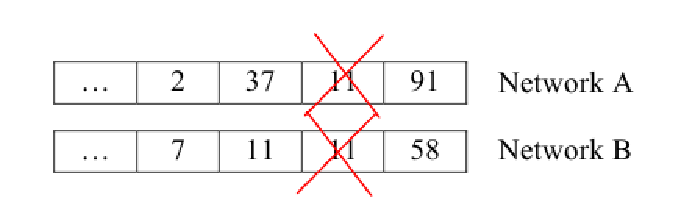
\includegraphics[width=9cm]{mm7_exercise1-1a_cdma.eps}
  \caption{Illustration of collision between two synchronous FH networks. The number denotes the frequency selected in that slot}
  \label{fig:mm7_exercise1-1a_cdma}
\end{figure}

\subsection{a)}
\textit{Find the probability that network A experiences a collision if there are two collocated networks A and B which are synchronous, as on \figref{fig:mm7_exercise1-1a_cdma}}
If the system is synchronous then there will be a collision if the two networks picks the same frequency. For M frequencies the probability will be the probability that B picks every other frequency. 
\begin{flalign}
 && P(coll) =& 1 - P(no coll)& \\
 && \left(1-\frac{M-1}{M}\right) =& \frac{1}{M}&
\end{flalign}


\subsection{b)}
\textit{Find the probability that network A experiences a collision if there are two collocated networks which are asynchronous, as on \figref{fig:mm7_exercise1-1b_cdma}}
\begin{figure}[!h]
  \centering
  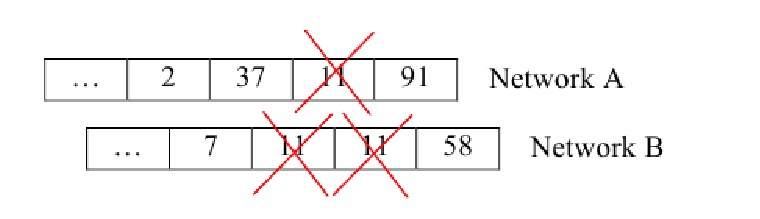
\includegraphics[width=9cm]{mm7_exercise1-1b_cdma.eps}
  \caption{Asynchronous FH networks.}
  \label{fig:mm7_exercise1-1b_cdma}
\end{figure}

If we call C1 the event of a network B causing a collision in the first overlapped time slot and C2 the event of said network causing a collision in the second overlapped time slot, then the probability of collision is:

\begin{flalign}
 P_{AsynColl} = P_{C1} + P_{C2} - P(C1\cap C2) = \frac{1}{M}+\frac{1}{M}-\frac{1}{M^{2}}
\end{flalign}

Which requires to substract $P(C1\cap C2)$ since the intersection between the events C1 and C2 is not empty. We also know, from the results in the previous problem, that the probability of the event C1 and C2 are equal and $P_{C1} = P_{C2} = \frac{1}{M}$.

\subsection{c)}
\textit{Let there be K$>$1 collocated networks, all of them asynchronous with each other. Find the probability that network A experiences a collision.}

The results from the previous problem show that $P_{AsynColl}$ is the probability of any network asynchronous to A, causes A to experiment collision. Thus if we have $K-1$ networks asynchronous to A, the probability of A experimenting a collision is:

\begin{flalign}
 P_{Coll-K-networks} = 1 - P_{NoCollisions}
\end{flalign}

Where $P_{NoCollisions}$ is the probability of the $K-1$ networks do not collide with A. Thus $P_{NoCollisions} = (1- P_{AsynColl})^{K-1}$. This leads to the probability of collision

\begin{flalign}
 P_{Coll-K-networks} = 1 - (1- P_{AsynColl})^{K-1}
\end{flalign}

\subsection{d)}
\textit{If the number of frequencies is M=80, the number of collocated networks is K=10, each packet carries 100 bytes and the duration of a slot (packet) is TP =50 $\mu$s, find the throughput in [bps] achieved in each network.}

The solution to this problem was computed using Matlab, where:

\begin{flalign}
 Throughput = (1 - P_{Coll-K-networks}) \cdot \frac{100 bytes}{50 \mu s} = 1.789 Mbytes/s
\end{flalign}
